\documentclass[12pt, twoside]{article}
\usepackage[letterpaper, margin=1in, head=30pt, headsep=0.1in]{geometry}
\usepackage[english]{babel}
\usepackage[utf8]{inputenc}
\usepackage{amsmath}
\usepackage{amsfonts}
\usepackage{amssymb}
\usepackage{tikz}
\usetikzlibrary{quotes, angles}

\usepackage{graphicx}
\usepackage{enumitem}
\usepackage{multicol}

%\usepackage{pgfplots}
%\pgfplotsset{width=10cm,compat=1.9}
%\usepgfplotslibrary{statistics}
%\usepackage{pgfplotstable}
%\usepackage{tkz-fct}
%\usepackage{venndiagram}

\usepackage{fancyhdr}
\pagestyle{fancy}
\fancyhf{}
\renewcommand{\headrulewidth}{0pt} % disable the underline of the header
\raggedbottom
\newif\ifmeta
\metatrue %print standards and topics tags

\title{Math AI Worksheet Generator and Formative Assessment System}
\author{Chris Huson}
\date{February 2021}

%\fancyhead[RE]{\thepage}
%\fancyhead[RO]{\thepage \\ Name: \hspace{3cm}}
%\fancyhead[L]{BECA / Dr. Huson / 10th Grade Geometry\\* 7 June 2019}
%
%\begin{document}
%\subsubsection*{13.7 Homework: Cross sections, distance applications}
%\fancyhead[L]{BECA / Dr. Huson / Geometry 03-Volume+angle-bisectors\\* pset ID: 34}

\begin{document}

\subsubsection*{6.3 Slope formula}
\begin{enumerate}

\item Find the slope of the line $\overleftrightarrow{AB}$, $A(2,1)$, $B(3,4)$. Use the formula and show the substitution step.
\begin{multicols}{2}
  $\displaystyle m = \frac{y_B - y_A}{x_B - x_A}$
    \vspace{2cm}
    \begin{flushright}
    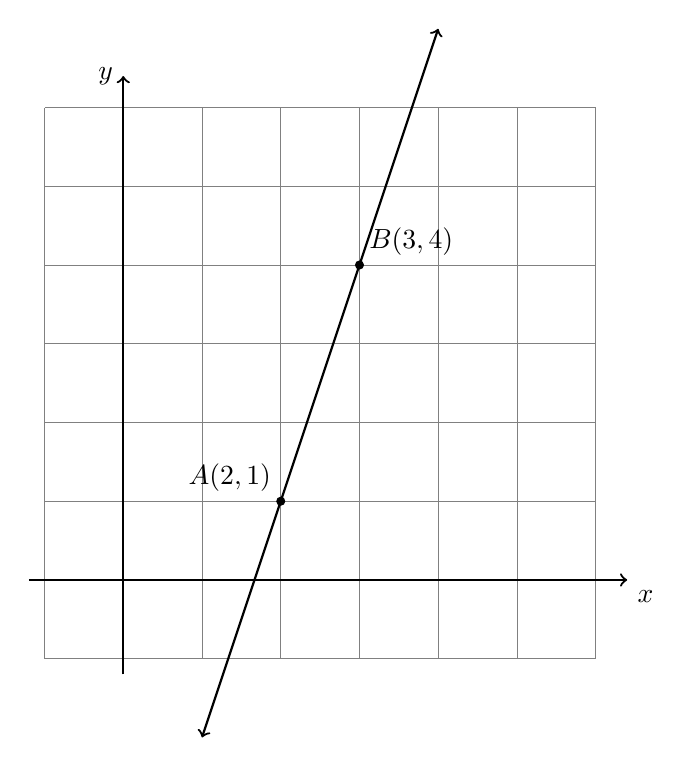
\begin{tikzpicture}[scale=1]
      \draw [help lines] (-1,-1) grid (6,6);
      \draw [thick, ->] (-1.2,0) -- (6.4,0) node [below right] {$x$};
      \draw [thick, ->] (0,-1.2)--(0,6.4) node [left] {$y$};
      \draw [fill] (2,1) circle [radius=0.05] node[above left] {$A(2,1)$};
      \draw [fill] (3,4) circle [radius=0.05] node[above right] {$B(3,4)$};
      \draw [<->, thick] (1,-2)--(4,7);
    \end{tikzpicture}
    \end{flushright}
\end{multicols}

\newpage
\item Plot the points and find the slope of the line $\overleftrightarrow{RS}$, $R(1,3)$, $S(3,4)$. Use the formula and show the substitution step. As a check, draw the line and count the rise and run.
\begin{multicols}{2}
  $\displaystyle m = \frac{y_S - y_R}{x_S - x_R}$
    \vspace{2cm}
    \begin{flushright}
    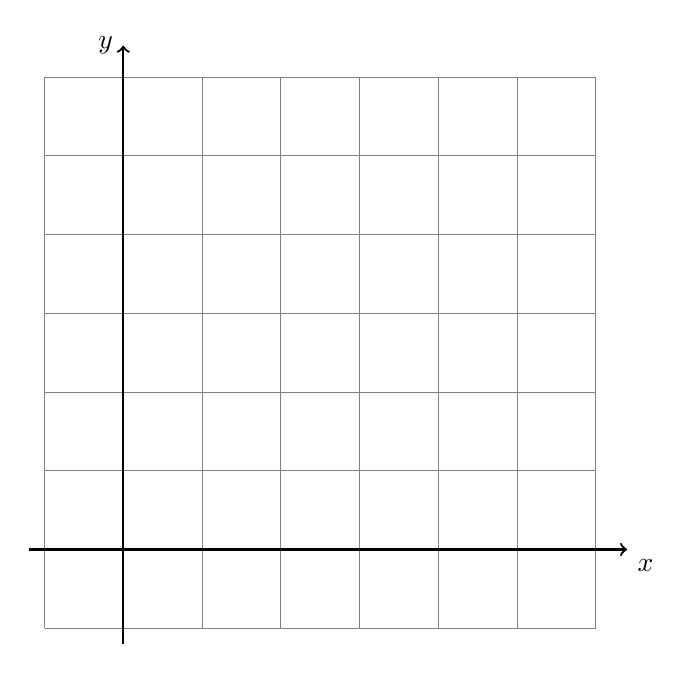
\begin{tikzpicture}[scale=1]
      \draw [help lines] (-1,-1) grid (6,6);
      \draw [thick, ->] (-1.2,0) -- (6.4,0) node [below right] {$x$};
      \draw [thick, ->] (0,-1.2)--(0,6.4) node [left] {$y$};
      %\draw [fill] (2,1) circle [radius=0.05] node[above left] {$A(2,1)$};
      %\draw [fill] (3,4) circle [radius=0.05] node[above right] {$B(3,4)$};
      %\draw [<->, thick] (1,-2)--(4,7);
    \end{tikzpicture}
    \end{flushright}
\end{multicols}

\newpage
\item Find the equation of the given line $\overleftrightarrow{AB}$, $A(0,4)$, $B(4,2)$.
\begin{multicols}{2}
    \begin{enumerate}[itemsep=1cm]
      \item Find the slope, $m$, showing the substitution step in the slope formula: \\[0.5cm]
      $\displaystyle m = \frac{y_B - y_A}{x_B - x_A}$\\[0.5cm]
      \item Write down the $y$-intercept.
      \item Write the equation of the line in the slope-intercept form\\[0.25cm]
      $y=mx+b$
      \end{enumerate}
    \begin{flushright}
    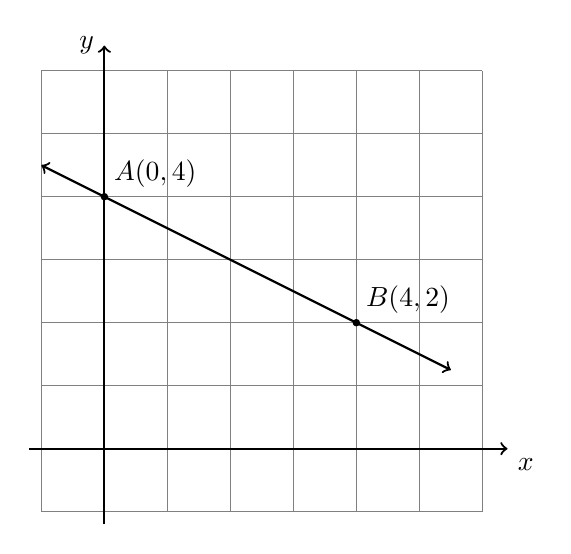
\begin{tikzpicture}[scale=0.8]
      \draw [help lines] (-1,-1) grid (6,6);
      \draw [thick, ->] (-1.2,0) -- (6.4,0) node [below right] {$x$};
      \draw [thick, ->] (0,-1.2)--(0,6.4) node [left] {$y$};
      \draw [fill] (0,4) circle [radius=0.05] node[above right] {$A(0,4)$};
      \draw [fill] (4,2) circle [radius=0.05] node[above right] {$B(4,2)$};
      \draw [<->, thick] (-1,4.5)--(5.5,1.25);
    \end{tikzpicture}
    \end{flushright}
\end{multicols}

\newpage
\item Complete each statement about linear equations.
\begin{enumerate}[itemsep=0.5cm]
  \item What is the slope of a horizontal line?
  \item What is the $y$-intercept of the line $y = 2x + 3$?
  \item What is the slope of the line $y = x - 5$?
  \item Which has an undefined slope, a vertical or horizontal line?
  \item What is the $y$-intercept of the line $y = -2x$?
\end{enumerate}

\newpage
\item Two parallel lines are shown in the graph, $p$ and $q$.
\begin{multicols}{2}
    \begin{enumerate}[itemsep=1cm]
      \item Find the slope, $m$, by counting squares across and up on the line. \\[0.5cm]
      $\displaystyle m = \frac{rise}{run}$\\[0.5cm]
      \item True or false: parallel lines have equal slopes.
      \item Write the slope of a line perpendicular to $p$ (the negative reciprocal).\\[0.25cm]
      $m_{\perp}=$
      \end{enumerate}
    \begin{flushright}
    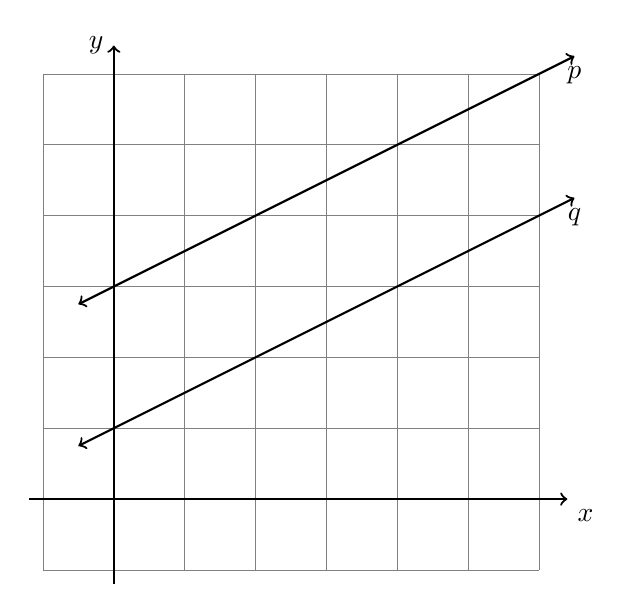
\begin{tikzpicture}[scale=0.9]
      \draw [help lines] (-1,-1) grid (6,6);
      \draw [thick, ->] (-1.2,0) -- (6.4,0) node [below right] {$x$};
      \draw [thick, ->] (0,-1.2)--(0,6.4) node [left] {$y$};
      %\draw [fill] (0,4) circle [radius=0.05] node[above right] {$A(0,4)$};
      %\draw [fill] (4,2) circle [radius=0.05] node[above right] {$B(4,2)$};
      \draw [<->, thick] (-0.5,2.75)--(6.5,6.25) node [below]{$p$};
      \draw [<->, thick] (-0.5,0.75)--(6.5,4.25) node [below]{$q$};
    \end{tikzpicture}
    \end{flushright}
\end{multicols}

\newpage
\item Write down the slope perpendicular to each slope (its negative reciprocal).
\begin{enumerate}[itemsep=0.9cm]
  \item If $m = 2$ then $m_{\perp}=$
  \item If $m = -3$ then $m_{\perp}=$
  \item If $\displaystyle m = \frac{2}{3}$ then $m_{\perp}=$
  \item If $\displaystyle m = -\frac{3}{4}$ then $m_{\perp}=$
\end{enumerate}

\newpage
\item Plot the $\triangle ABC$ with vertices $A(2,2)$, $B(5,1)$, and $C(6,4)$. \\[0.5cm]
Find the slopes of $\overleftrightarrow{AB}$ and $\overleftrightarrow{AC}$. Is the triangle a right triangle?
  \begin{center}
    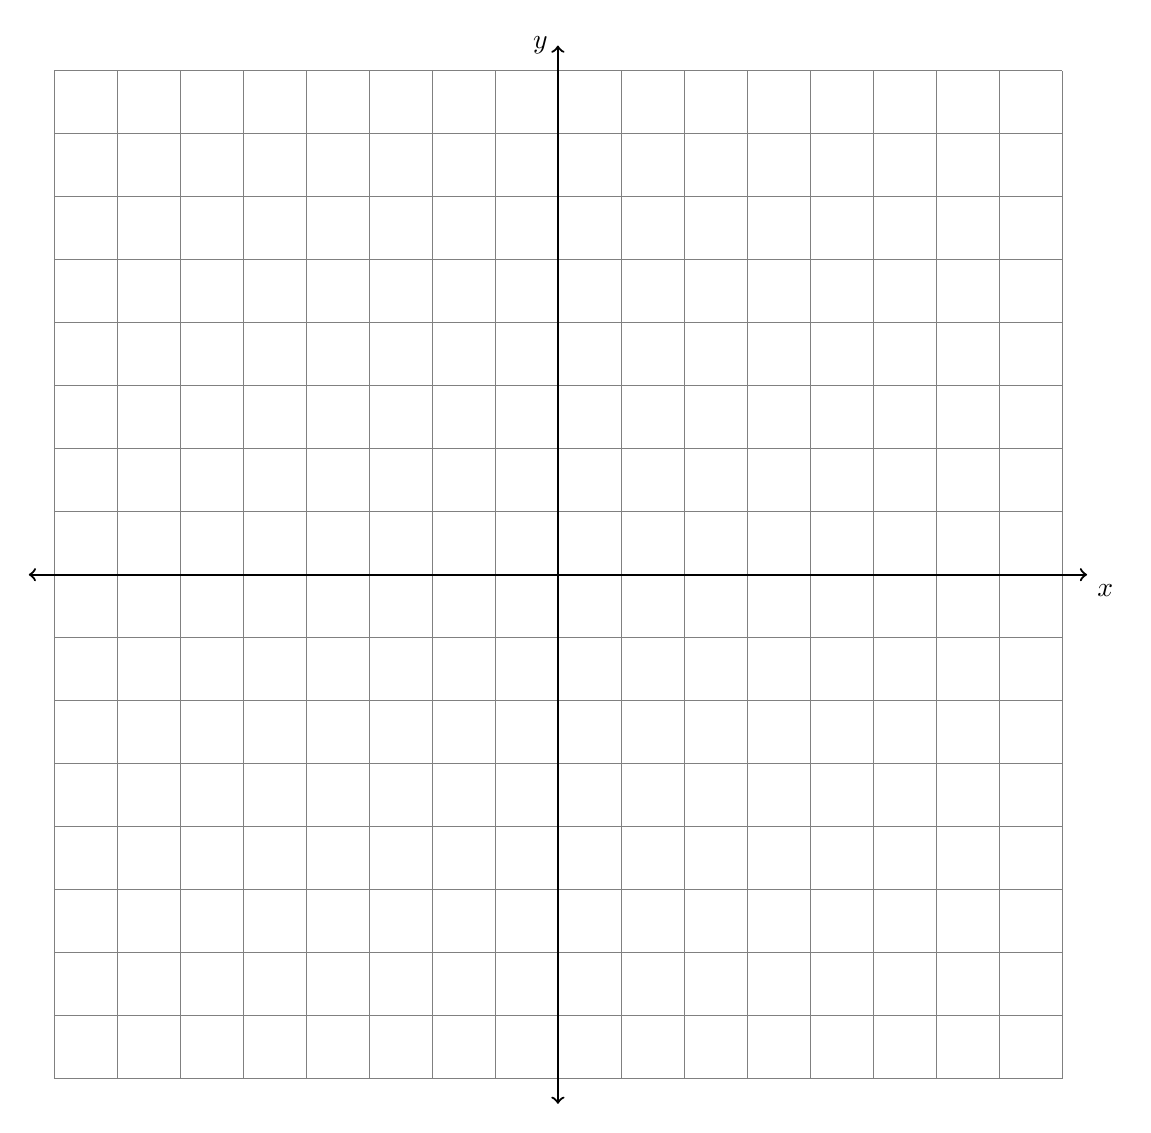
\begin{tikzpicture}[scale=0.8]
      \draw [help lines] (-8,-8) grid (8,8);
      \draw [thick, <->] (-8.4,0) -- (8.4,0) node [below right] {$x$};
      \draw [thick, <->] (0,-8.4)--(0,8.4) node [left] {$y$};
      %\draw [thick] (2,2) node[below] {$A$}--
      %  (5,1) node[right] {$B$}--
      %  (6,4) node[above right] {$C$}--
      %  cycle;
    \end{tikzpicture}
    \end{center}

\newpage
\item Is the point $C(4,2)$ on the line $l: y=\frac{1}{2}x+1$? \\[0.5cm]
Support your answer with \emph{both} algebra (substitute $C$'s coordinates into the equation) and geometry by graphing the line and point $C$.
  \begin{flushright}
  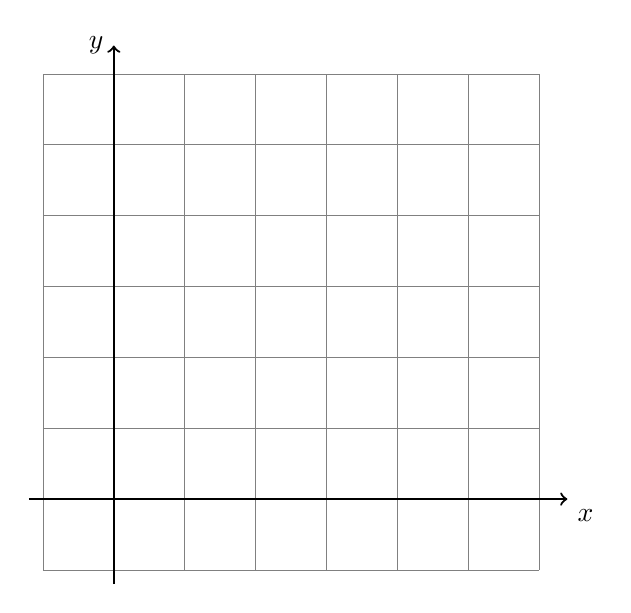
\begin{tikzpicture}[scale=0.9]
    \draw [help lines] (-1,-1) grid (6,6);
    \draw [thick, ->] (-1.2,0) -- (6.4,0) node [below right] {$x$};
    \draw [thick, ->] (0,-1.2)--(0,6.4) node [left] {$y$};
  \end{tikzpicture}
  \end{flushright}
    

\newpage
\item Plot the same triangle as problem 7 using Geogebra/classic. Paste an image of your work in this Classkick slide from the clipboard or by using the ``camera'' tool.\\[0.25cm]
Spicy: measure the slopes of the relevant triangle sides and the measure of $\angle B$

    
\end{enumerate}
\end{document}

\newpage
\item A point labeled $C$ and vector $(1,3)$ are shown Geogebra/classic. Identify the following objects and tools.
  \begin{enumerate}
    \item Circle the vector
    \item Make an ``X'' where to click for the menu ``Name \& Value'' that will label point $C$ as an ordered pair.
    \item Mark with an arrow the menu where the ``Translate by vector'' tool is found.
  \end{enumerate}
  \begin{flushright}
    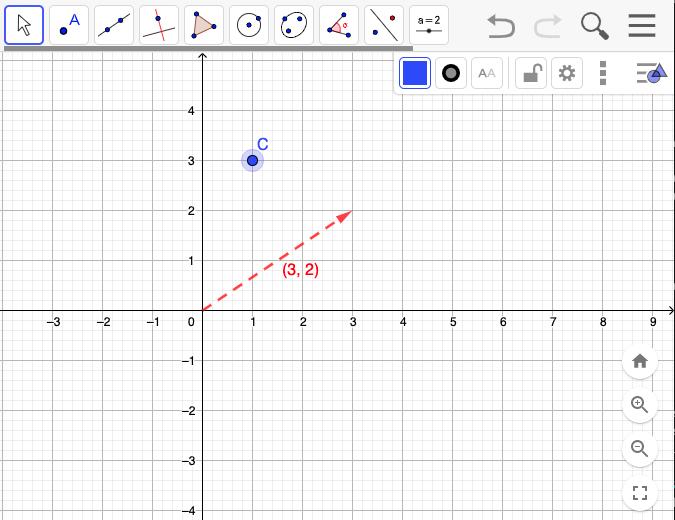
\includegraphics[width=6in]{5-11Geogebra_toolbar.png}
  \end{flushright}
